\chapter{Implementation}
TODO!


\section{System Design}
The software developed for this thesis is a stand-alone point-cloud viewer that allows the user to interact with the point cloud. The application consists of three strands that are executed in parallel. 


\section{Functional Programming}
\label{sec:funprog}

Functional programming is a paradigm that views every expression as a mathematical function. The result of each expression is either an elemental datatype or a functional type. A core difference to other programming paradigms is the equality of function and data, such that functions can be used as input for other functions and have a distinct type defined by its parameters and result. A simple example of a function in \verb|F#|: 

\begin{lstlisting}[language=FSharp]
let square (i : float) : float = i * i 
\end{lstlisting}

This function is of type \verb|float -> float|. It takes a \verb|float| as input and returns a \verb|float|. This functional type can be used as input parameter as well. A definition for a function that takes a function as parameter looks as follows: 

\begin{lstlisting}[language=FSharp]
let compute (i: float)(f : float -> float) : float = f i
\end{lstlisting}
Its type is \verb|float -> (float -> float) -> float| and is used as such: 
\begin{lstlisting}[language=FSharp]
let result = compute 10.0 square
\end{lstlisting}

\verb|result| is an expression that executes the \verb|compute| function with arguments $10.0$ of type \verb|float| and \verb|square| of type \verb|float -> float|. Even tough this is just a simple example, it showcases the strength of functional programming.  Using functions as input allows the user to create complex and dynamic computations with ease. 
\\

Functional programming tries to mitigate mutations as much as possible. Mutations, e.g. change of a variable's state, introduces several risks to the program. While each expression in a function context is mathematically defined, such that parameter space and result space are fully defined, now values are returned that the program does not expect, thus mitigating undefined behavior. Moreover, mutation of an expression can change the behavior of expressions that depend in the mutated field, thus changing the result, without changing the parameter. 
\\

\verb|F#|\cite{FSharp} is a functional programming language developed and maintained by Microsoft\cite{Microsoft}. F\# is fully integrated into the .NET framework\cite{DotNet} and is built upon the Common Language Infrastructure\cite{CLI}, thus allowing it to use resources written in other languages, such as C\#\cite{CSharp}. Even though F\# is a functional language, it also supports object-oriented programming, such that types with member functions can be used as well. 


\section{Aardvark}

The Aardvark platform\cite{aardvark} is a functional-first incremental rendering engine in active development at the VRVis Zentrum für Virtual Reality und Visualisierung\cite{vrvis}. It is an implementation of research results on the field of incremental rendering \cite{, lazy} and semantic shader composition\cite{haaser2014cosmo, haaser2014semantic}. 

The key feature of the Aardvark platform is incremental rendering. In a conventional engine, updates are performed periodically. each object in the scene is reevaluated, even tough the simulation or user-input did not yield any changes. Incremental rendering counters this overhead by reacting to changes, such that only parts that depend on changed values are reevaluated. This section describes some of Aardvark's key features that are used throughout this thesis. Section \ref{sec:adaptive} shows the language-specific constructs on how to build adaptive blocks that react to changes. A \textit{scene graph} represents an object hierarchy in the scene. Section \ref{sec:isg} describes the composition of a scene graph using only a handful of lines of code. 

 
\subsection{Adaptive - IMod - transact}
\label{sec:adaptive}

As mentioned in Section \ref{sec:funprog} mutations are often the cause of undefined behavior and bugs. In order to introduce state-changeable variables into a functional environment, Aardvark provides the \verb|IMod<'a>| type. This generic type is a wrapper around a certain value, whose value might change over time. The platform contains an extensive implementation for a three-dimensional transformation, called \verb|Trafo3d|. In order to listen to changes for such a transformation, a type \verb|IMod<Trafo3d>| is needed. The following example shows the composition of a model transformation from a position, scale, and rotation, all of which can might their value over time. 

\begin{lstlisting}[language = FSharp]

let position     : IMod<V3d> = ... 
let scale         : IMod<V3d> = ... 
let rotation    : IMod<V3d> = ...

let trafo : IMod<Trafo3d> = 
    adaptive {
    
        let! sc  = scale
        let! rot = rotation
        let! pos = position
        
        
        let S = Trafo3d.scale sc
        let R = Trafo3d.Rotation rot
        let T = Trafo3d.Translation pos
        
        return S * R * T
    }
\end{lstlisting}

The \verb|adaptive| block allows the system to keep track of the state of all IMods that are accessed using the \verb|let!| operator. The result of the adaptive block, again, is an IMod<Trafo3d>. If one of the accessed IMods changes its value, the code below, including the line of the \verb|let!| is reevaluated using the previously caches values. 
\\

To actively change a value, a subtype of \verb|IMod<'a>|, \verb|ModRef<'a>| is needed. The type \verb|ModRef<'a>| contains the functionality to allow changes to the value, thus causing reevaluation. All state transactions are collected and executed sequentially, thus reducing the number of reevaluations and circumventing race-conditions. In order to achieve that each change must be wrapped in a \verb|transact| type. 
The following example uses the Aardvark-specific mouse callback function to trigger a reevaluation based on mouse movement. The Move-callback is called each time the mouse moves and provides the user with the old position and the new position. The difference on the x-axis controls the y-value of the rotation. 

\begin{lstlisting}[language = FSharp]
let mouse : IMouse = ...

let rotation : ModRef<V3d> = Mod.init V3d.OOO

mouse.Move.Values.Add(fun (oldPos : PixelPosition, newPos : PixelPosition) -> 
    let delta = 
			newPos.NormalizedPosition.X - oldPos.NormalizedPosition.X
    let angle = delta * 2.0 * Math.Pi
    
    let newRotation = 
			rotation.GetValue() + V3d(0.0, angle, 0.0)
    
    transact(fun () -> Mod.change rotation newRotation)
    )
\end{lstlisting}

The \verb|rotation| can then be used within an \verb|adaptive| block like an \verb|IMod|. 
\\
Transactions are usually used to handle user input. However, asynchronous computations that produce results in parallel use transactions as well in order to mitigate race conditions and notify the system. 


\subsection{Scene graph composition}
\label{sec:isg}

A scenegraph (\verb|ISg|) contains all information that is needed to render this object. A common paradigm in functional programming is to split functionality from data, such that the functions that utilize this data, are stored in a different namespace than the data. In combination with the pipe operator ($|>$) clean and easy-to-read code can be produced. The following example showcases the composition of an \verb|ISg|. 

\begin{lstlisting}[language = FSharp]

// Transformations
let trafo:	IMod<Trafo3d> = ... 
let view:	IMod<Trafo3d> = ...
let proj:	IMod<Trafo3d> = ...

// IndexedGeometry contains triangles to render
let geometry : IndexedGeometry = ...

// The renderpass for this scenegraph
let renderPass : RenderPass = ...
// The shader (surface) to render the geometry with
let shader : IMod<ISurface> = ...
// Create scenegraph
let sg = geometry	|> Sg.ofIndexedGeometry
                    |> Sg.trafo trafo
                    |> Sg.viewTrafo view
                    |> Sg.projTrafo proj
                    |> Sg.pass renderPass
                    |> Sg.surface shader
\end{lstlisting}

The field \verb|sg| represents a scene graph with transformations, geometry, shader and render pass without the need of complicated constructors or setter functions. Furthermore, an own implementation of \verb|ISg| can easily extend the functionality without reimplemented procedures for this specific type. 


\subsection{Out-of-core capabilites}
The Aardvark platform already implements functionality to handle out-of-core data. The type \verb|Database| provides means to store data. A chunk of data that is stored on in this database is called \verb|thunk<'a>| where \verb|'a| is the type of the data to be stored. The following code shows hot to create a \verb|thunk<'a>|. 

\begin{lstlisting}[language = FSharp]
	let db : Database	= ...
	let data : 'a 	= ...
	
	let stored : thunk<'a> = db.ref data
\end{lstlisting}
When a thunk is loaded from the database its content is not loaded into memory yet. Only when accessing the data directly, it is loaded into memory. The data is held in memory as long as the thunk lives. Therefore it is crucial to keep track of unused thunks and dispose them regularly, thus freeing memory. 


\section{Functional Out-of-core Octree}

Chapter \ref{chap:octree} already provides information on the capabilities of the octree. This section describes implementation details of the octree's structure using out-of-core mechanics and custom parametric functions for convenient octree queries. 


\subsection{Structure}

The octree's out-of-core capability is managed by an interleaved structure of thunks. Each \verb|OctreeNode| contains an array of points. However, the array is not stored directly, it is stored as a \verb|thunk<Point[]>|. It's children are stored as an array of thunks (\verb|thunk<OctreeNode>[]|). The points are stored as a single thunk, the reason for storing the node's children in separate thunks is to not load all children into memory when only a subset of children is accessed. Other information such as the centroid, density, an rkd tree, and the detected primitive shapes are stored as thunks as well. 


\subsection{Elemental functions}

The interaction methods described in Section \ref{chap:interactions} heavily rely on the efficient collection of octree nodes that fulfill certain criteria, thus a set of routines is implemented that can easily be parameterized and reused. \verb|F#| collections contain several functions that use a lambda function as input and perform this function on elements in the collection. Some examples are \verb|map, filter| and \verb|choose|, all of which takes two arguments, an array and a function that takes an element as input. Even though the octree is not generic, such functions are implemented in a similar way, in order to provide efficient query functions for the octree. 


\subsubsection{Filter}

A common procedure in functional programming is filtering. Filtering is performed on a collection and returns the set of elements of this collection for which the decision function is \verb|true|. Filtering an octree is similar. However, the decision must be made if to use the current node and if to traverse the children as well, as children may be desired, where the parent is not. 
The function's definition looks as follows: 

\begin{lstlisting}[language = FSharp]
let filter (decisionFun : OctreeNode -> GridCell -> int[] -> bool*bool) (tree: Octree) : (Octree)= ...
\end{lstlisting}

The decision function takes as input the octree node, it's grid cell and its unique path in the octree as an array of indices. It returns a tuple of \verb|bool|, deciding whether to use this node and whether to traverse the children. The result of this operation is a new tree that only contains the nodes that are filtered. For the case that a parent node is not filtered, but some of its children are, an empty placeholder node is used instead to preserve the octree's structure. 


\subsubsection{Map}

Usually, the \verb|map| function is used for generic data structures to create a projection for each element and returns a data structure of the same type with the projected elements. Since the octree is not generic, the \verb|map| function returns the projection for each node of the octree as an array of \verb|'T| where \verb|'T| is the type of the projection. 
The functions's definition looks as follows: 

\begin{lstlisting}[language = FSharp]
let map (projection : OctreeNode -> GridCell -> int[] -> 'T) (tree: Octree) : ('T[])= ...
\end{lstlisting}

Contrary to the filter function, the \verb|map| function does not return a new octree since the type of the projection must not necessarily be hierarchical. Therefore an array of \verb|'T| is returned instead. 


\subsubsection{Choose}

A similar task to filtering is the choose function. However, instead of returning the filtered values directly, the decision function also maps the values to the desired type \verb|'T|. The decision function uses the same input as the decision function for filtering. Its return type is a tuple that consists of a \verb|Option<'T>| and a \verb|bool|. The option type is used to introduce null-mechanics into the functional context. An option can either be \verb|Some value| or \verb|None|. If the \verb|choose| function's returned type is \verb|Some value|, its value is filtered, the \verb|bool| value decides whether or not to traverse the children. 
The function's definition looks as follows: 

\begin{lstlisting}[language = FSharp]
let choose (decisionFun : OctreeNode -> GridCell -> int[] -> Option<'T>*bool) (tree: Octree) :('T[]) = ...
\end{lstlisting}


\begin{figure}[h]
    \centering
    \subcaptionbox{ \label{fig:octreeFilter}}{%
        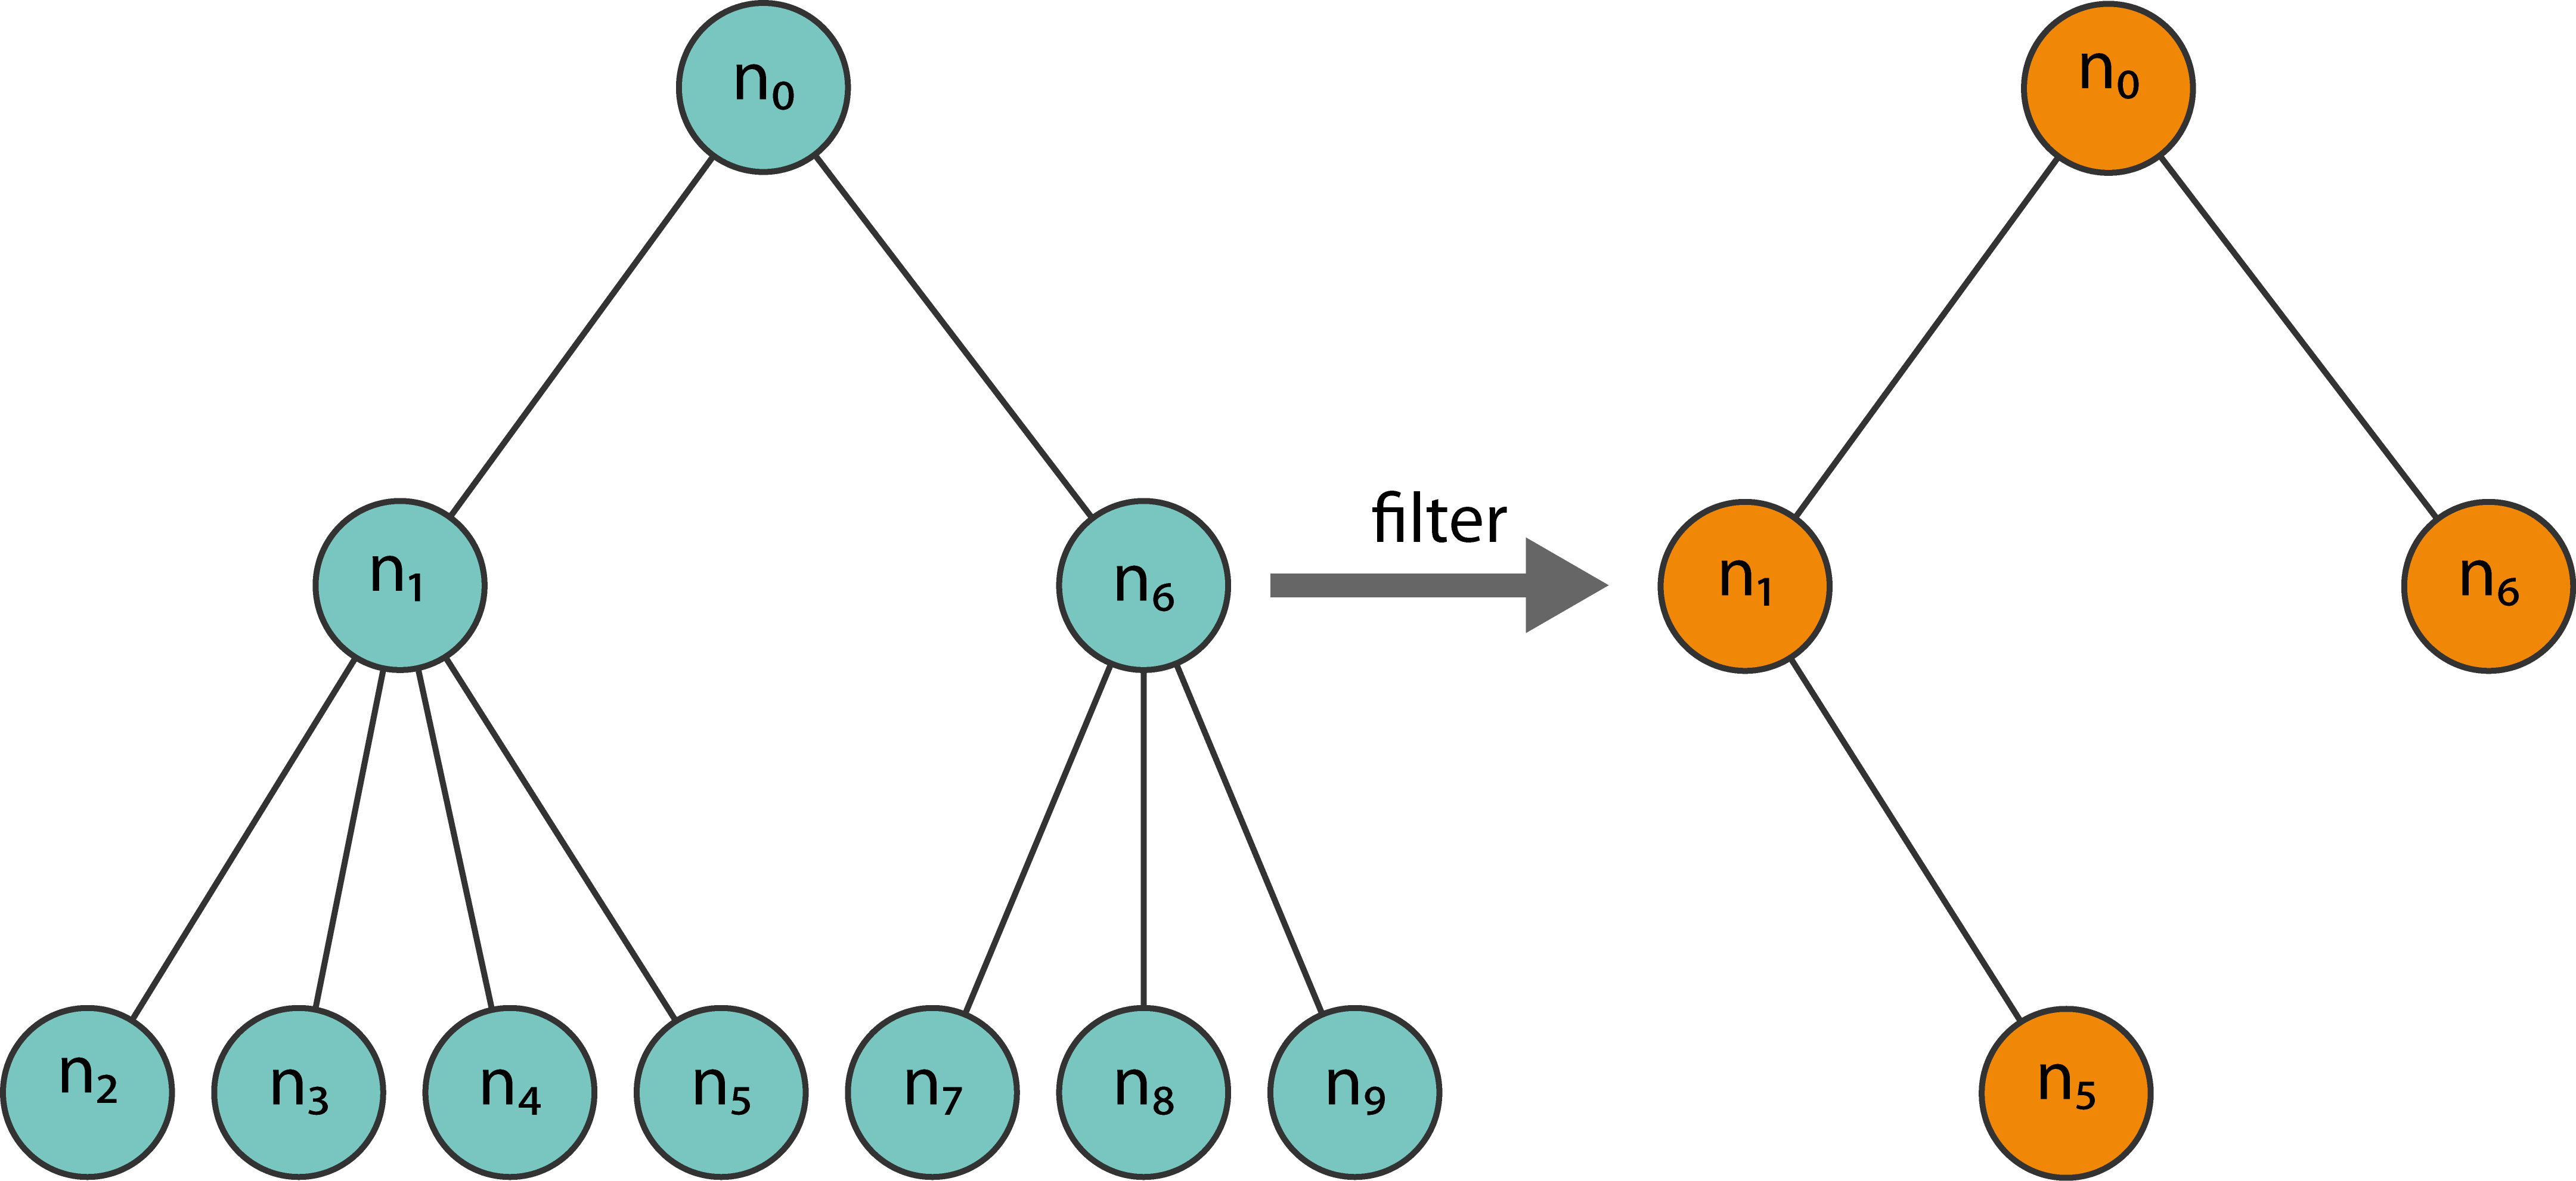
\includegraphics[width=0.55\textwidth]{Implementation/octreeFilter.png}%7
        }\par\medskip
    \subcaptionbox{ \label{fig:octreeMap}}{%
        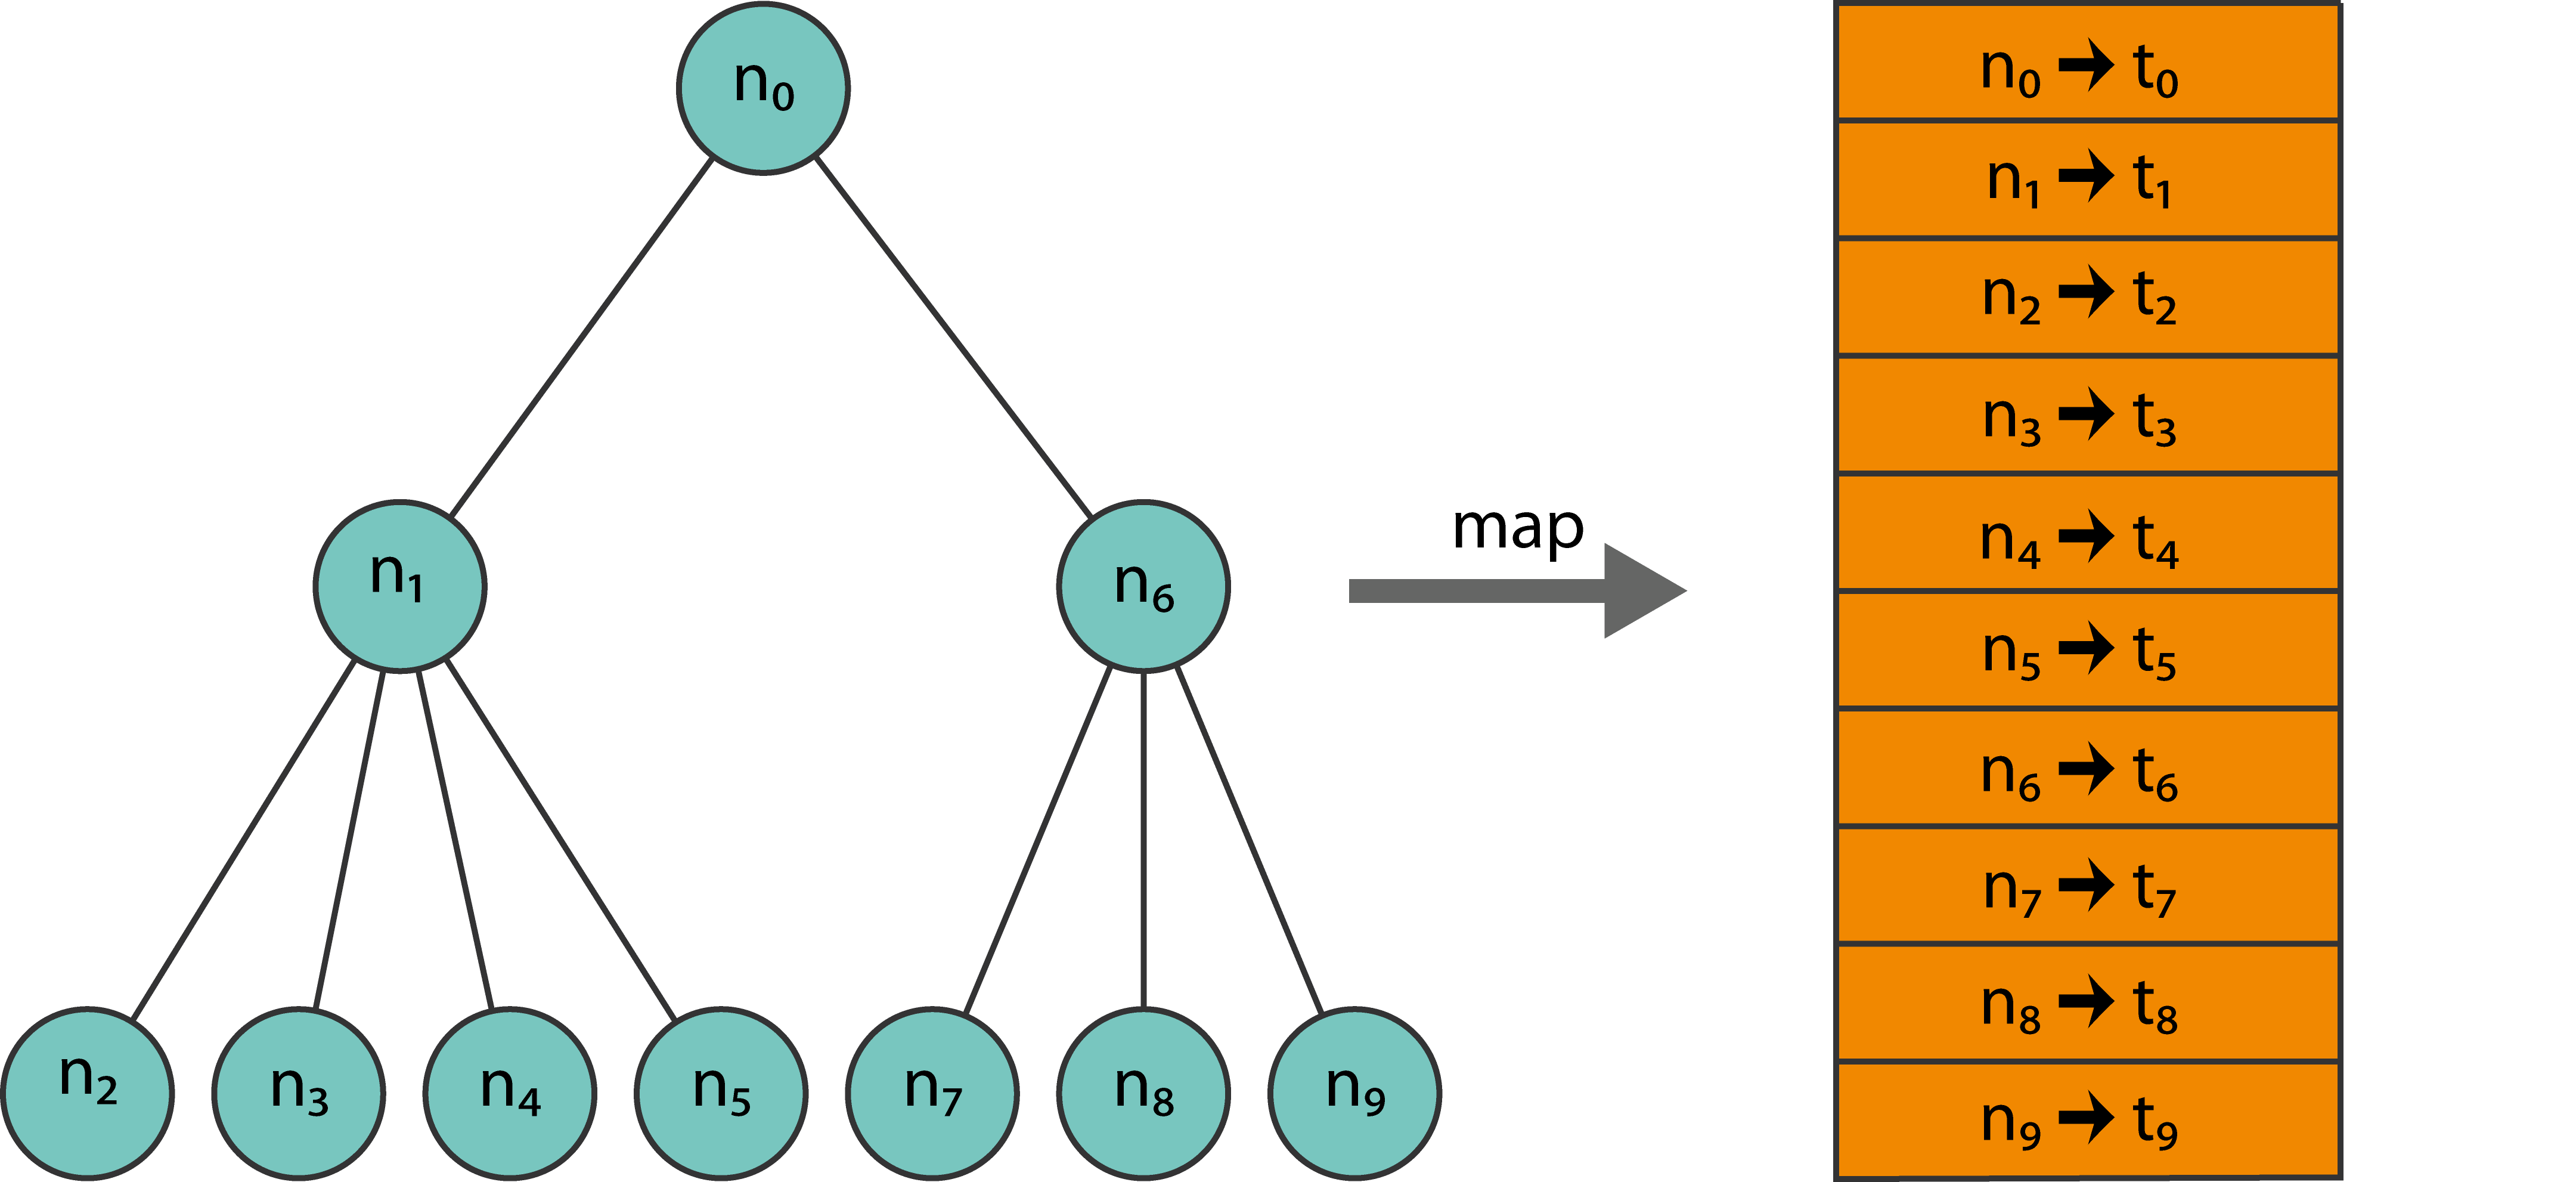
\includegraphics[width=0.55\textwidth]{Implementation/octreeMap.png}%
        }\par\medskip        
    \subcaptionbox{ \label{fig:octreeChoose}}{%
        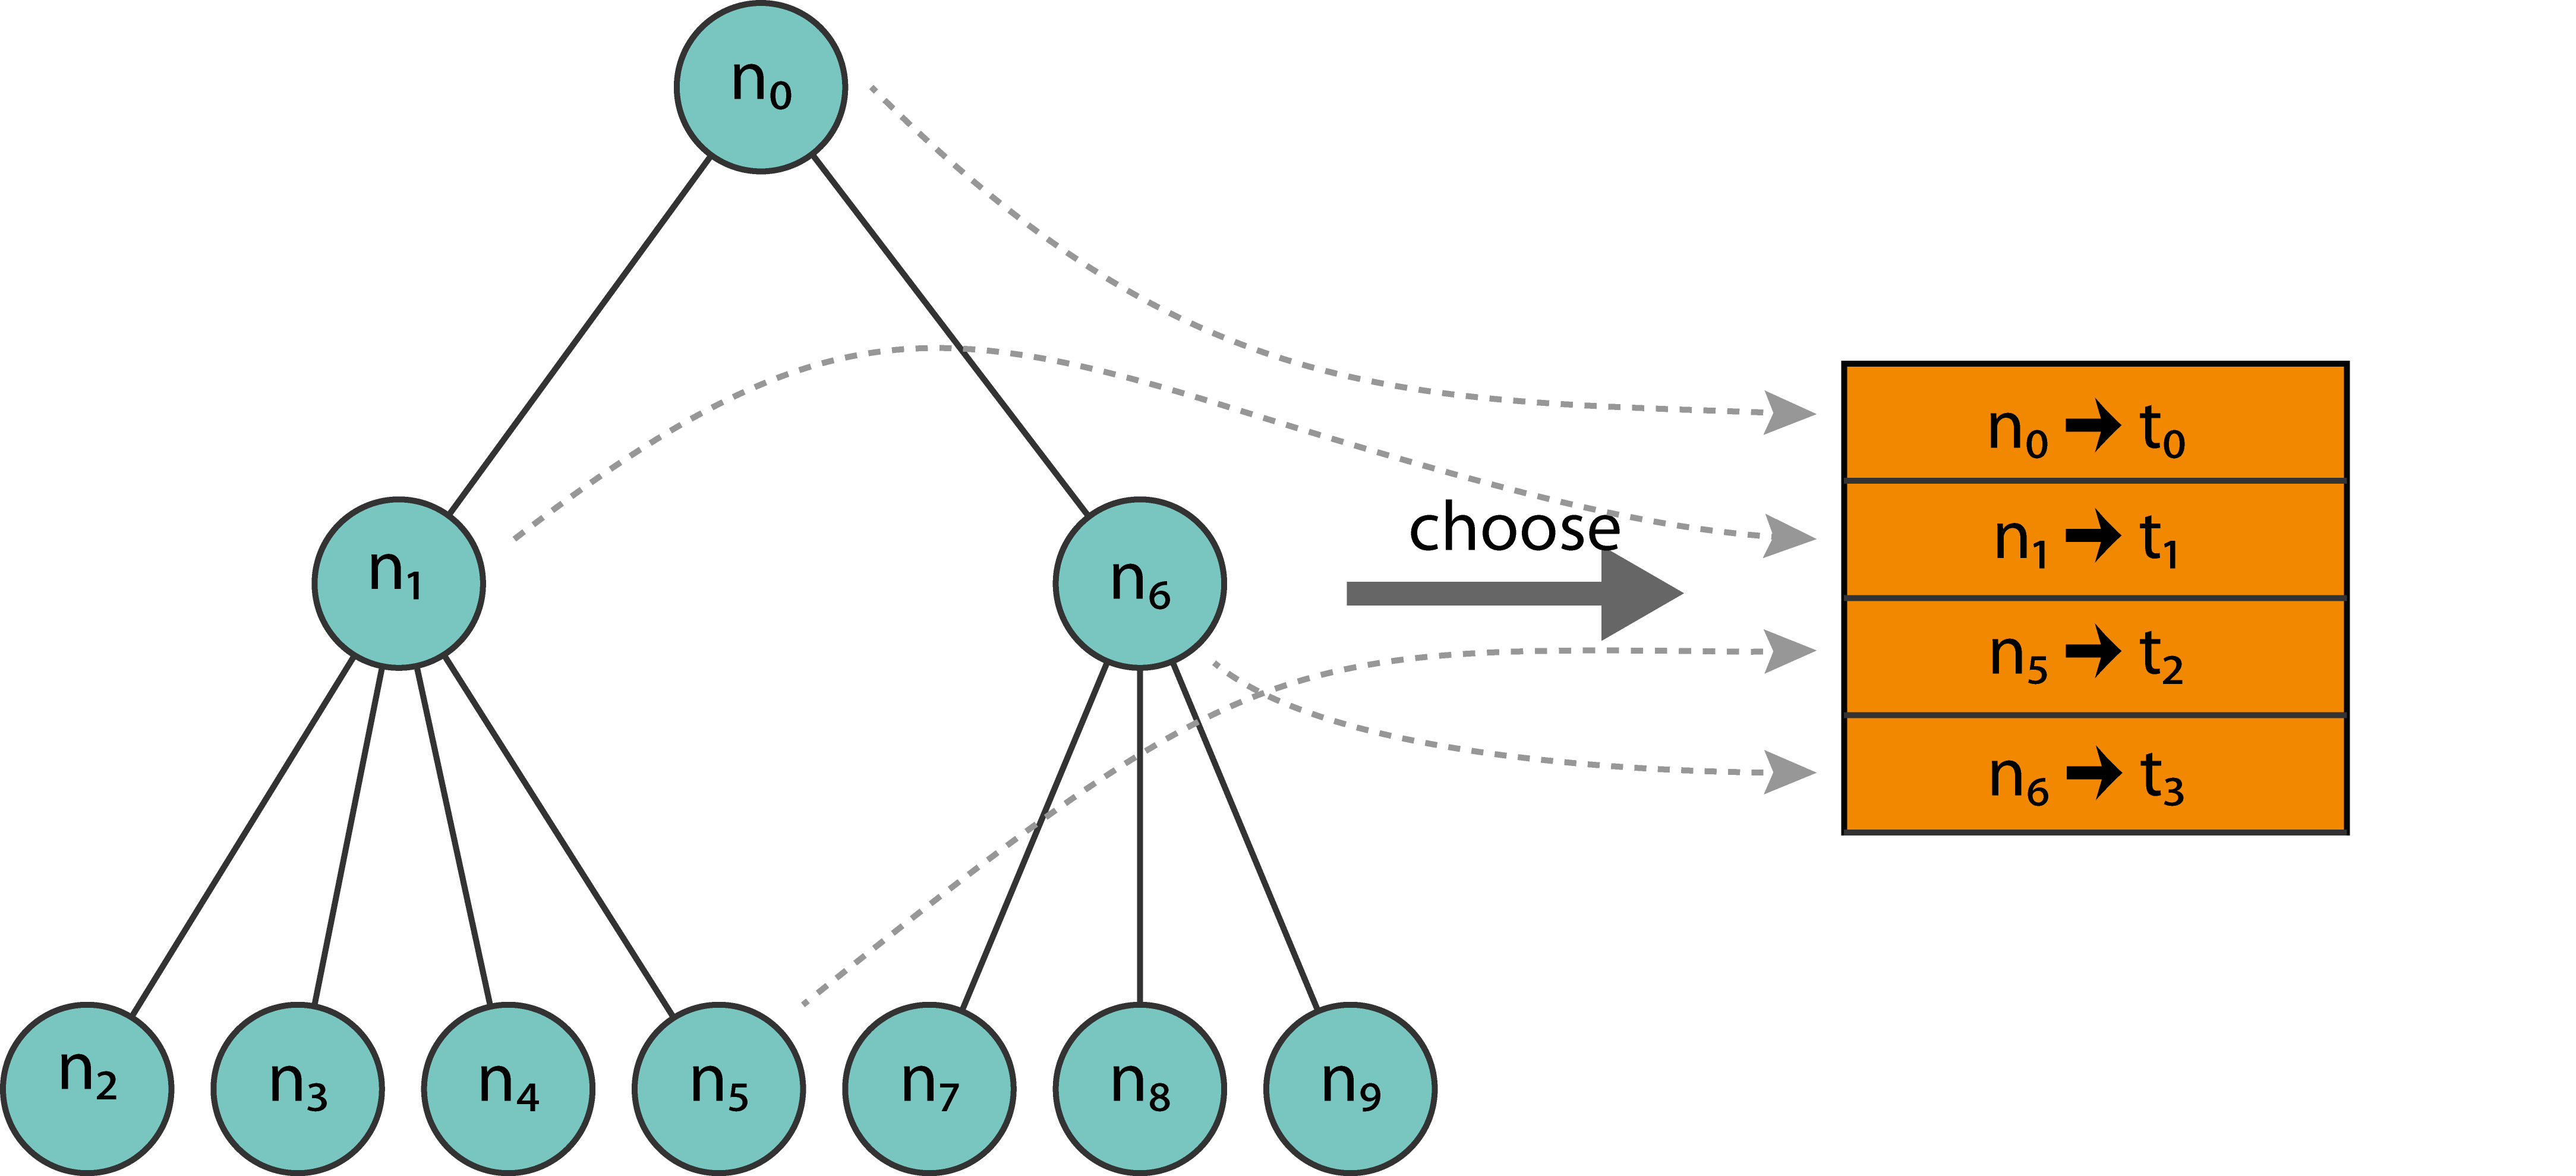
\includegraphics[width=0.55\textwidth]{Implementation/octreeChoose.png}%
        }
    \caption{This figure shows an exemplary octree, on which the filter, map and choose function is applied. In (a) the filter function creates a new octree that only contains the nodes that are filtered. (b) shows the result of the map function. Each node in the octree is projected to a new type $t_{i}$ and the result is returned as an array. (c) shows the choose function. Only nodes are returned that fulfill the decision function and are projected to a new type $t_{i}$. }
    \label{fig:octreeFuns}
\end{figure}


Figure \ref{fig:octreeFuns} shows the described functions and its' effects on an exemplary octree. The \verb|filter| function returns a new octree, the\verb|map| function returns an array of projected types, the \verb|choose| function is a combination of \verb|filter| and \verb|map| such that only those projections are returned that are of interest. 


\subsubsection{Replacing nodes}

As mutations introduce side effects that can lead to bugs, instead of changing information within an octree node, a new node is created containing the new information. The old node might still be in use in a different thread, thus race conditions are possible when mutating values. When information changes in an octree node, a new \verb|thunk| is created that stores the new content onto the disc, the old \verb|thunk| is discarded when it is not used anymore. The newly created node has a distinct position that is determined by the path in the octree. The octree is traversed recursively to find the position of the node. 
\\
When the recursion is resolved, The content of all ancestor nodes has changed as well, since one of the children is a new node. Therefore, for each ancestor, a new node is created too, containing the new content. Since the root changes as well, as the replaced node is a successor of it, a new octree is constructed each time a node is replaced. This octree, however, contains mostly the data of the old octree, with the exception of the replaced node. 

\begin{figure}[h]
    \centering
    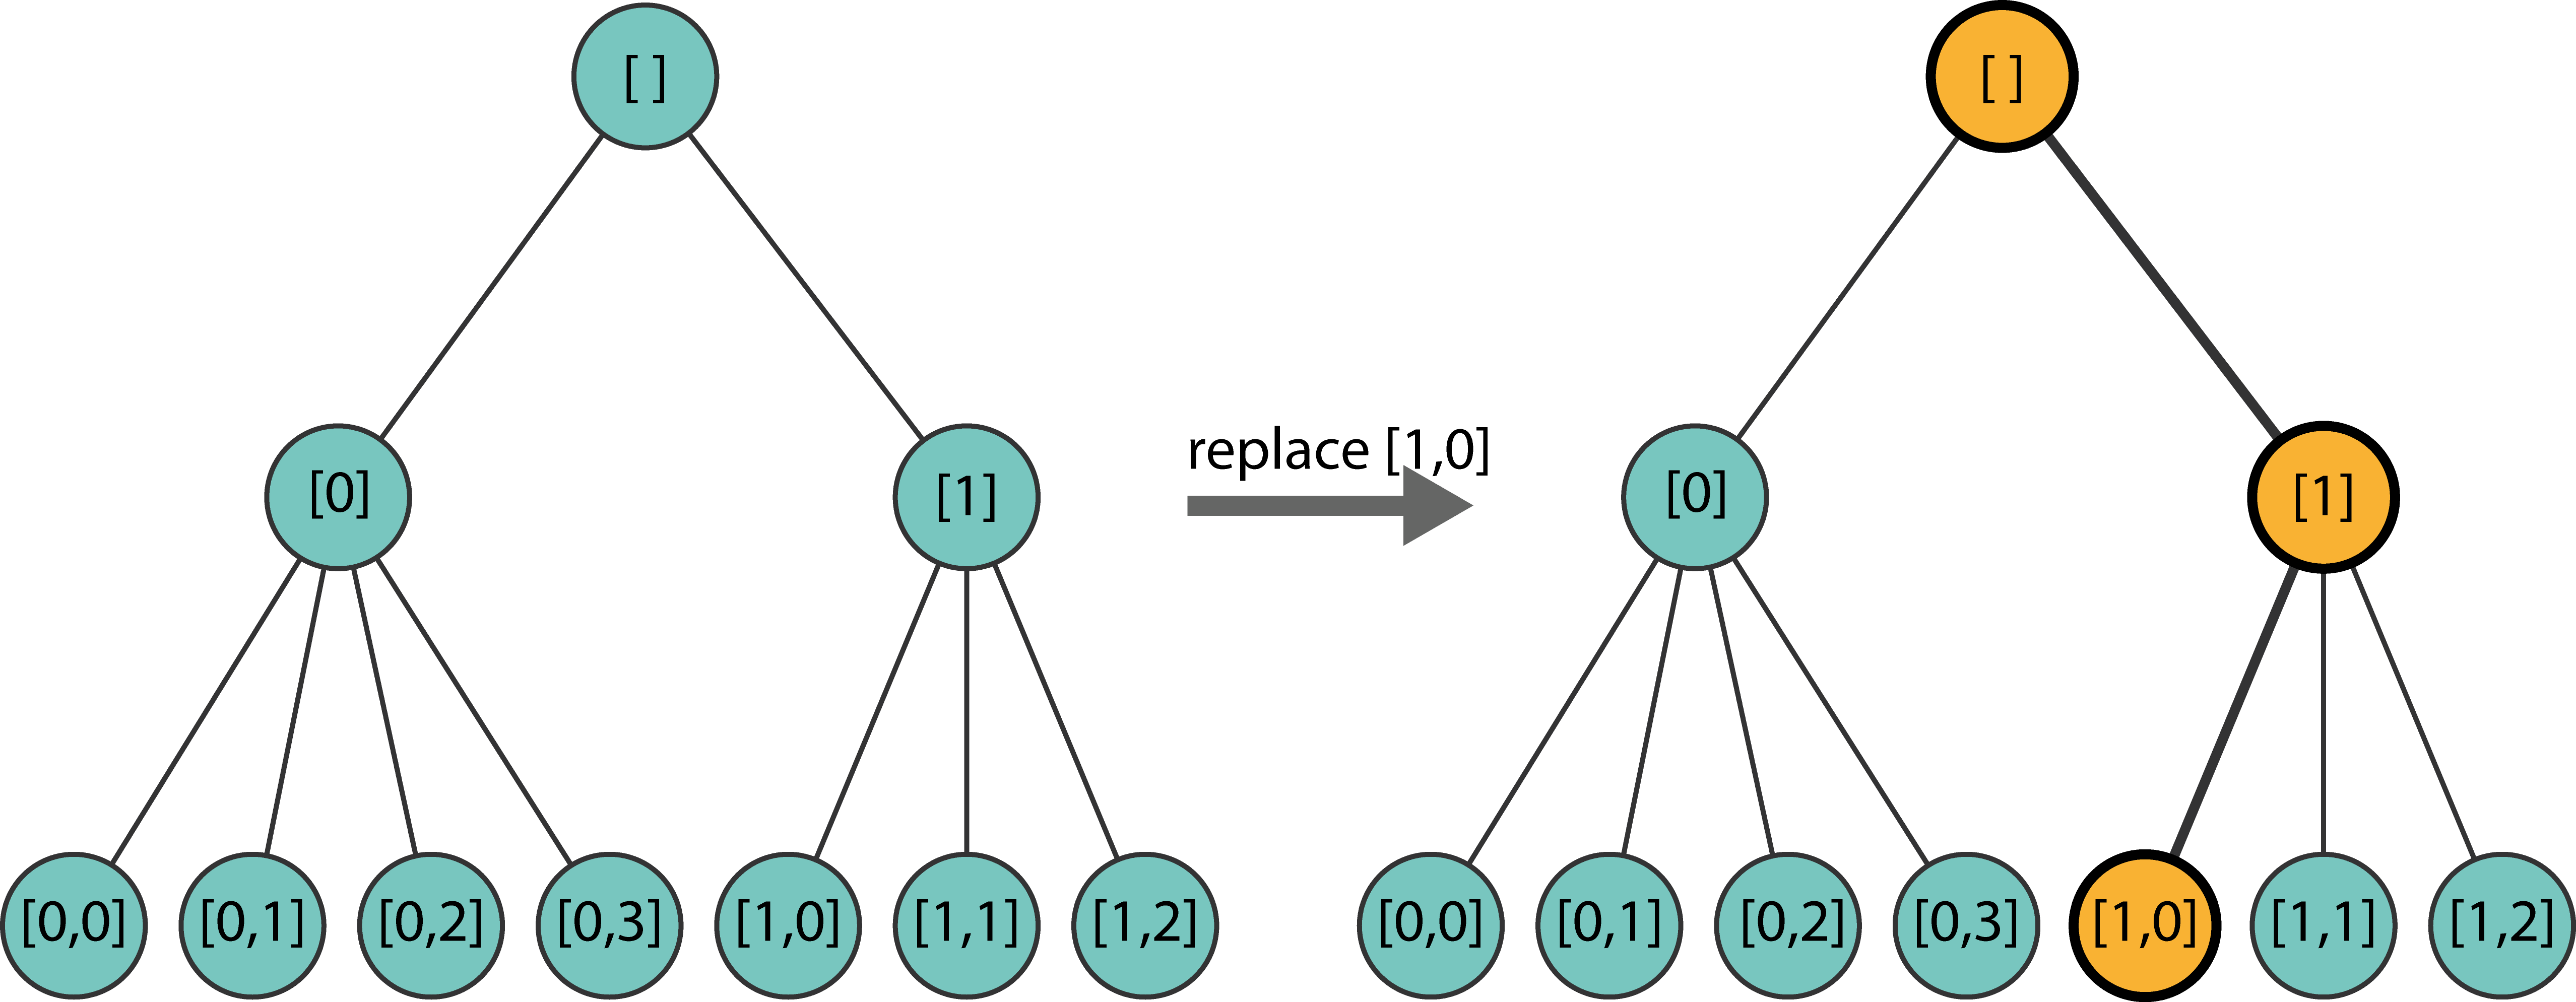
\includegraphics[width=0.8\textwidth]{Implementation/octreeReplace.png}
    \caption{Replacing an octree node subsequently changes the node's ancestors as well. The left tree shows the original octree, the right tree is the new octree after the node [1,0] was replaced. The replaced node is highlighted with a red border, all nodes that changed due to the replacement are colored in orange. }
    \label{fig:octreeReplace}
\end{figure}

Figure \ref{fig:octreeReplace} shows an example on the replacement of a node. The nodes are labeled with their paths in the octree in order to uniquely identify them. The node with label \verb|[1,2]| is replaced, thus all ancestors in the octree are changed as well since the node got a new child. All nodes that changed, thus creating a new octree, are colored in orange. 


\subsection{Culling}

Culling directly uses the octree's \verb|filter| function to create a new octree that only contains nodes that are currently rendered. The culling function performs view-frustum culling as well as the \verb|level-of-detail| culling heuristic based on the node's size and distance to the nearplane. 


\begin{figure}
    \centering
    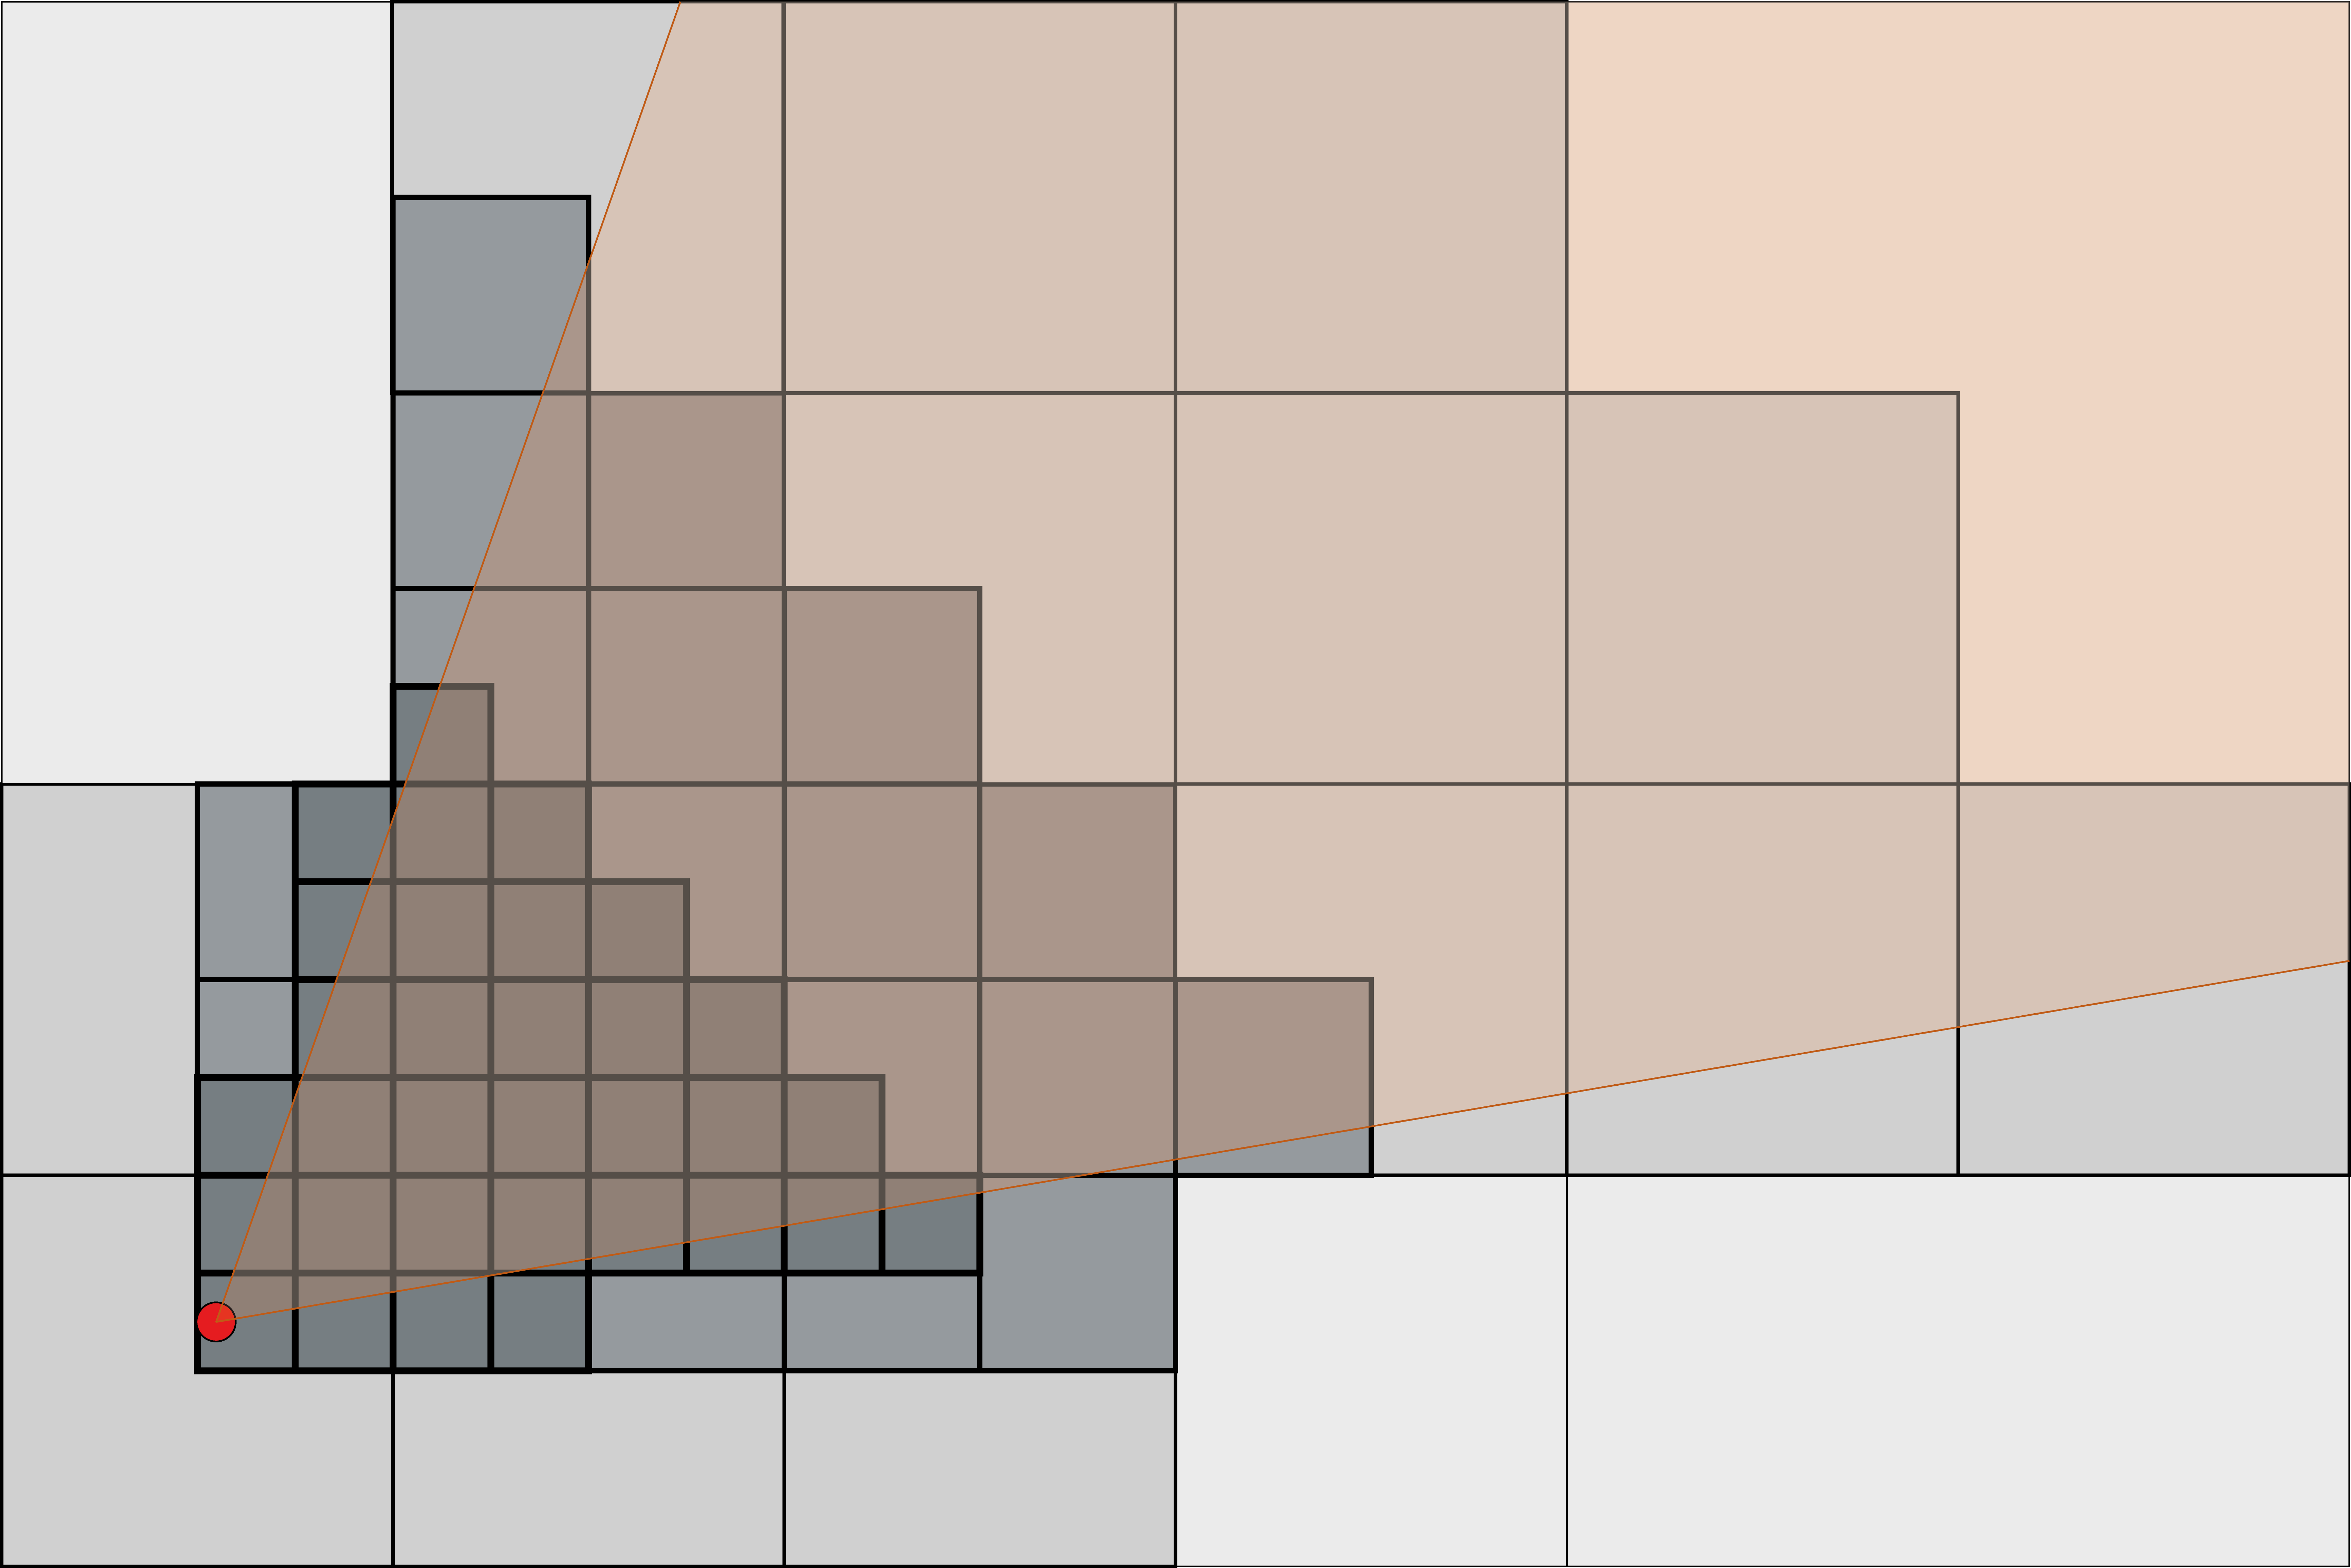
\includegraphics[width=0.8\textwidth]{Implementation/octreeCulling.png}
    \caption{An exemplary culling is performed on a tree. Octree nodes that are darker with a thicker edge have a higher \textit{leve-of-detail}. Only close to the camera (red), the nodes with the highest \textit{level-of-detail} are rendered. Nodes that are outside the view frustum(orange) are discarded. }
    \label{fig:octreeCulling}
\end{figure}

Figure \ref{fig:octreeCulling} shows an exemplary culling performed on a tree. The \textit{level-of-detail} decreases for nodes that are further away from the camera and only those nodes are used that intersect the view frustum. 

\subsection{Diff}

As discussed in Section \ref{sec:renderHorizon}, the render horizon is the set of nodes that are still rendered, and at least one of the children is not. The \textit{Shape-Assisted Local Level-of-Detail Increment} interaction, described in Section \ref{sec:lod_increment}, uses the render horizon to collect a set of nodes that are beyond the horizon in order to draw additional points onto the screen. This set of nodes is obtained by the octree's \verb|diff| function. 
\\
Let $t1, t2$ be two octrees where $t2$ is a sub tree of $t1$. The function \verb|diff t1 t2| returns all nodes from t1, whose parents exist in t1 and t2, but the node itself only exists in t1.
\\
The \verb|diff| function takes nodes that are in the first octree and not in the second octree. In the case of the \textit{Shape-Assisted Local Level-of-Detail Increment}, interaction $t1$ is the complete octree, $t2$ is the culled octree that only contains nodes that are rendered. 
\\
Additionally, not only the children are collected, but depending on a depth value, the children's successors are collected as well. 


\subsection{Raycast}

An octree is an ideal data structure to accelerate ray casting. The hierarchical structure ensures that only a minimum set of nodes is tested for intersection. If the ray does not intersect the parent's bounding box, it does not intersect the children's bounding boxes as well. The raycast on the octree can be performed with logarithmic cost. The raycast is implemented using the octree's \verb|choose| function with a decision function that performs the intersection with the bounding box and returns a \verb|RaycastHit| structure containing all necessary information on the raycast hit. 


\section{Sequential Computation Applicator}

The octree receives changes on a regular basis from multiple sources in this application. The shape detection coroutine continuously inserts detected primitive shapes into the octree, resulting in a new octree every time. User interactions change the point set by selecting regions of interest. To synchronize the octree access, locking mechanics can be used. However, such mechanics can get confusing easily, especially when the application grows. 
\\
All changes to the octree are dependent on the state of the octree that, in the meantime, may be changed by an operation from a different thread. Furthermore, since a new octree is created every time, the result of an operation may be overlooked when a second operation starts while the first operation has not yet finished. All subsequent operations depend on the result of the previous operation, thus a structure is needed that handles such dependent operations. 
\\
The \verb|Sequential Computation Applicator| is a structure that provides a synchronized way of processing sequential operations. The applicator's functionality is synchronized such that multiple threads can dispatch operations on the octree. The \verb|Sequential Computation Applicator| is a wrapper around a \verb|ModRef<'T>| that invokes changes on the value regularly. 
In this case, the type of the applicator wraps around a \verb|ModRef<Octree>|. 

All dispatched operations are sequentially processed and the \verb|ModRef|'s value is changed after an operation is completed, thus notifying the Aardvark engine. 
The applicator provides the interfaces to dispatch an operation, as well as to dispatch an operation with high priority, thus enqueueing the operation on the front. 

\begin{lstlisting}[language = FSharp]

    member public this.DispatchPrioritized(computation : 'T -> 'T) (timeout : int) (timeoutCallback  : unit -> unit) : unit = ...

    member public this.Dispatch(computation : 'T -> 'T) (timeout : int) (timeoutCallback  : unit -> unit) : unit = ...
   
\end{lstlisting}

The type \verb|'T| is the generic type of the \verb|Sequential Computation Applicator|, in this case, it is \verb|Octree|. A computation is dispatched that takes a \verb|'T|, and projects it to a new \verb|'T|. The input parameter on execution is the current value of the octree. 
Additionally, an operation can be shut down after a defined timeout in milliseconds. If this is the case the \verb|timeoutCallback| is invoked to allow clean up and error handling. 


\section{Multi-Threaded Environment}

Multi-threading can be achieved on multiple scales, depending on the tasks need. The application uses three basic threads that run in parallel. 
\\
The Aardvark rendering engine, combined with the \verb|IMod| evaluation system and user interactions build the main thread of the application. One pitfall of the \verb|IMod| system is that it only reacts to changes in the system, however, to invoke procedures after a certain time without changes is not possible directly. 
\\


The \textit{user-guided shape detection} from Section \ref{sec:user_guided_sd} relies on the camera not changing for a certain amount of time. 
A separate thread continuously checks for changes and, if a shape detection should be performed and dispatches the computation to the applicator thread, 
\\
The \textit{sequential computation applicator} performs changes dispatched to it in an sequential order. It receives computations from several thread and performs them in the background. The thread transacts the changes to the main thread once a computation has finished. 

\begin{figure}
    \centering
    \includegraphics[width=0.6\textwidth]{Implementation/multiThreading.png}
    \caption{The main thread controls the rendering, mod evaluation and interactions. Point selections from interactions are handed to the applicator thread. The shape detection is invoked by a separate thread and dispatched on the applicator thread as well.  }
    \label{fig:multiThreading}
\end{figure}

As Figure \ref{fig:multiThreading} shows, multiple thread are dispatching computations to the applicator thread. However, only this thread transacts changes to the main thread. The shape detection invoker thread works independently of the main thread. 


The second technique of parallelization that is used is to identify similar tasks that are executed in parallel for multiple instances, such as per-point or per-node computations. As long as shared resources are not written into, such tasks can easily performed in parallel. The input is an array of elements and a task to be executed for each element. The result is an array of the results of the computation for each element. The function's signature looks as follows: 
\\
\begin{lstlisting}[language = FSharp]
module Parallel = 
  let map (computation : 'T1->'T2)(array : 'T1[]) : 'T2[]= ...
\end{lstlisting}
The technique is realized as an parallel implementation of f\#s \verb|map| function for arrays. 

\verb|Parallel.map| is used when point or node conversions are needed, such as projecting points to screen space or calculating the distances of points to a shape. 


\section{Point-Cloud Rendering}

Modern point cloud's often contain several billion points. Current GPUs are not able to handle such amounts of point. The culling heuristic in Section \ref{sec:renderHorizon} already reduces the set of nodes to a handful that are manageable for the GPU and can be drawn in real time. However, the point data may still be located on the hard drive and must be loaded into memory. 
\\
The Aardvark platform already contains a \textit{level-of-detail} point cloud rendering system that can handle out-of-core datasets. The rendering system uses a cache to store nodes that were rendered previously. Once a frame is redrawn, all nodes that are rendered are collected and for new nodes the data must be loaded into the memory. New nodes are added to the cache, nodes that are not used in this, are kept in the cache until the memory consumption requires to remove unused data. For each node new to the cache, a thread is started to load the point data into memory. The frame is drawn even tough not all nodes are loaded. The frame is redrawn once the outstanding data is loaded onto the GPU, thus popping effects occur when the view changes drastically. 
\\
\\
Mathematically, a point has no a extent, therefore it cannot be depicted directly. A common way to draw points is to identify them as splats of certain size and shape. In this thesis the points are represented by a sphere imposter. For each point, a camera-aligned quad is created in a geometry shader, whose size is the diameter of the sphere, pixels that are outside the radius of the sphere are discarded. 
\\
Popping effects occur when when the view changes and overlapping imposters change their order. To counter such popping effects, the sphere is given a depth displacement that extrudes a sphere in world space, such that the depth value follows the curvature of the sphere, causing the imposters to intersect properly. Figure \ref{fig:point_sprites} shows a direct comparison of using spheres and circular splats. 


\begin{figure}
\centering
\subcaptionbox{ \label{fig:picking_raycast}}{%
  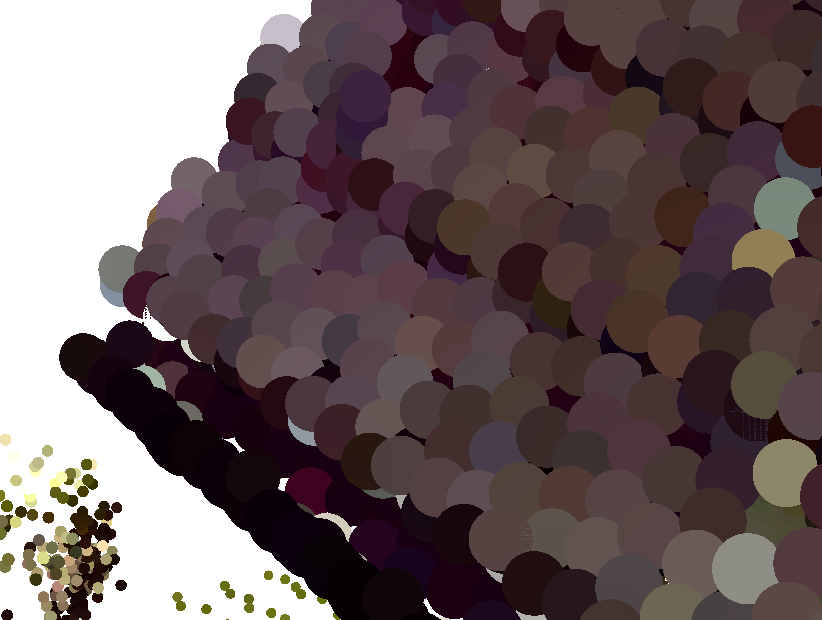
\includegraphics[width=0.48\textwidth]{Implementation/pointCircles.png}%7
  }
\subcaptionbox{ \label{fig:picking_conecast}}{%
  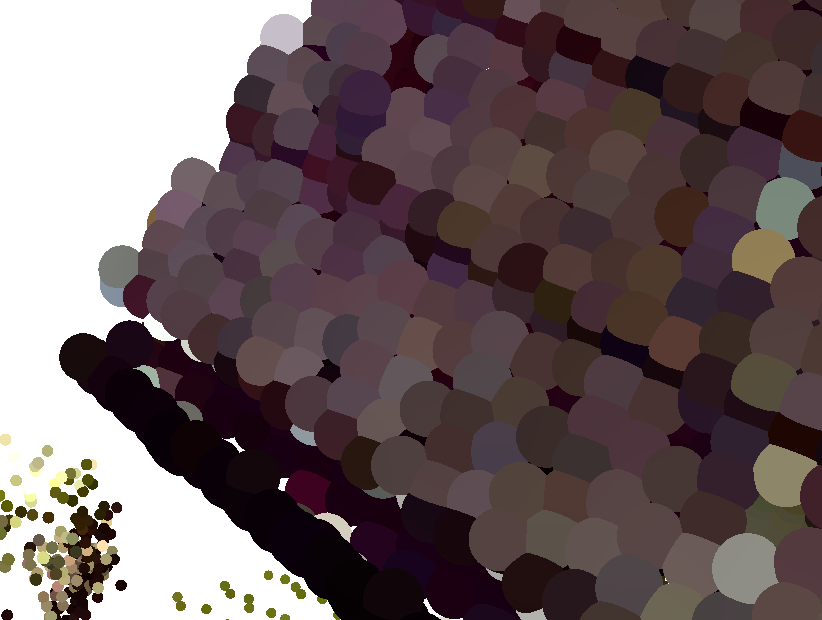
\includegraphics[width=0.48\textwidth]{Implementation/pointSpheres.png}%
  }
  
\caption{This figure shows a direct comparison of using (a) circular splats and (b) sphere imposters with depth displacement. In (b) the intersections between points are visible due to the spherical shape, whereas points that are little below other points are almost completely occluded.  }
\label{fig:point_sprites}
\end{figure}

 
\section{Interaction Workflow}
\section{Benchmarks}